\section{Simulação}
\subsection{Dataset}
\frame{
    \frametitle{Detalhes do dataset}
    \begin{itemize}
    \item Projeto Reality Mining, realizado entre 2004 e 2005 no
    laboratório MIT Media.
    \vspace{.4cm}
    \item 94 usuários monitorados usando seus telefones celulares.
    \vspace{.4cm}
    \item Log de informações:
    \begin{itemize}
        \item Ligações realizadas e recebidas.
        \item ID bluetooth de aparelhos próximos
        \item Identificador da torre associada ao sinal do celular.
    \end{itemize}
    \end{itemize}
} 

\subsection{Redes sociais}
\frame{
    \frametitle{Rede}
    O dataset não fornece uma visão completa da rede.
    \begin{figure}
    \centering
    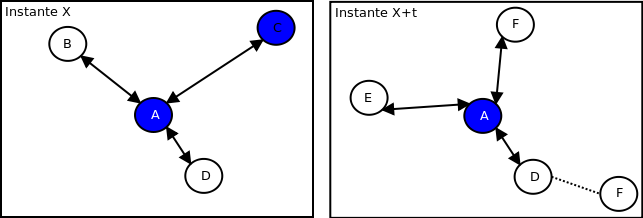
\includegraphics[width=\textwidth]{../doc/img/diagramas/redeSocial.png}
    \caption{Diagrama que ilustra a dinamicidade da rede considerada na
    simulação}
    \label{fig:dinamicidade}
    \end{figure}
}

\subsection{Codificação em rede}
\frame{
    \frametitle{Codificação em rede: Rede Aleatória de Codificação}

    \begin{itemize}
      \item \textbf{Codificação em rede}: Técnicas de processamento de dados com o objetivo de aumentar a capacidade da rede.
      \vspace{.4cm}
      \item \textbf{Rede Aleatória de Codificação:} \\ Cada mensagem contém: \\
        $\rightarrow$ Vetor de codificação (gerado aleatoriamente) e combinado com vetores anteriores\\
        $\rightarrow$ Mensagem codificada\\
      \vspace{.4cm}
      \item Decodificação depende de pacotes com informações codificadas (linearmente independentes).
    \end{itemize}


}

\frame{
    \frametitle{Codificação em rede: Rede Aleatória de Codificação}
    \begin{figure}
      \centering
      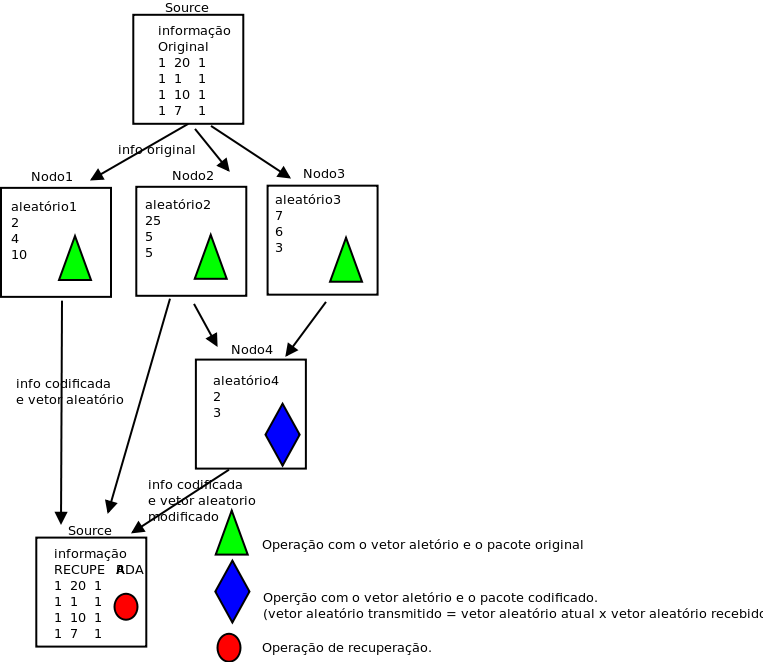
\includegraphics[scale=.3]{../doc/img/diagramas/netCodingDiagram.png}
    \end{figure}

}
\subsection{Detalhes da execução}
\frame{
    \frametitle{Algoritmos}
    \begin{itemize}
    \item \textbf{Epidêmico:} Cada nodo que recebe uma mensagem repassa a seus vizinhos (broadcast), caso algum de seus vizinhos ainda não possui essa informação.
    \vspace{.6cm}

    \item \textbf{SocialRoute:} Cada nodo somente repassa a informação caso o nodo atual ou algum dos vizinhos seja amigo do destinatário.
    \end{itemize}
}

\frame{
    \frametitle{Parâmetros}
    \begin{itemize}
    \item 1666 nodos, entre participantes do experimento e aparelhos
    percebidos por estes participantes
    \vspace{.6cm}
    \item Período considerado: 1 semana
    %explicar do custo computacional, e tals
    \end{itemize}
}
